\chapter{Atomic Magnetometry\label{ch:magnetometry}}
\small

 In the following chapter, there will be given an introduction into the quantum mechanical
structure and interactions of a Rb atom with special focus on the hyperfine structure and the Zeeman splitting of the energy levels in an external magnetic field. In the second section of this chapter, the principle of atom-light interactions including optical pumping
will be explained. After introducing basic concepts of alkali atom quantum mechanics, the phenomenology of nonlinear magneto-optical rotation (NMOR) will be discussed, which is the basis for the operation of an atomic magnetometer as it will be used for the nEDM setup

\section{Ground state structure of Rb }
\label{S:2} 
Alkali-metal atoms have single electron in their outer shell. For this reason they are often used for optical pumping. Alkali-metal atoms have a nuclear spin.
 Because of the nuclear spin the energy level of these alkali atom becomes complicated. For example rubidium has Z = 37 where the first 36 electrons are in closed sub-shells and so their total angular momentum is zero. 
The ground state structure of the Rb atom is n = 5, l =0~(s-state), and j = 1/2, i.e, $5^2S_{1/2}$. The lowest excited states (l~=1) are the
 5p states. According to quantum theory of angular momentum
these 5p states have total electron angular momentum J = L + S where L is
the orbital angular momentum and S is the electron spin angular momentum. For the ~$5^2S_{1/2}$~ and $5^2P_{1/2}$ ~ states of~ $^{85}{Rb}$,  which has nuclear angular momentum I = 5/2,  the allowed values of F are ($5/2$ - $1/2$) = 2 ~and~ 5/2 + 1/2 = 3. When atoms absorb light, they must absorb both energy and angular
momentum in the transition from the ground state to an excited state. The ~$5^2P_{1/2}$~
state is separated from the ~$5^2S_{1/2}$~ state by an energy corresponding to 795 nm wavelength, it is called the
D1 line. Transmission corresponding to the energy difference between the ~$5^2S_{1/2}$~ and~ $5^2S_{1/2}$ levels of rubidium is termed the D2 line; its wavelength is roughly 780 nm\cite{doe:website}. For a D1-transition, the excited state F can occupy the states $F = 2$ or $F = 3$.
The U of Winnipeg Rb atomic magnetometer is based on exciting the D1-line transition by optical pumping.  Linearly polarized laser beam is used to induce transitions of electrons from one energy level to another via optical pumping. In this case, the laser beam is tuned to the transition frequency and of sufficient power to perturb the equilibrium distribution of the ground state energy levels\cite{}. 


\section{Atom-light interaction} 

In this section, an introduction into the principle of atom-light interactions will be given. Starting with different polarization modes of laser light and their impact on optical pumping, the concept of frequency /amplitude modulation of the pump laser light will be given.

\subsection{Polarization of laser light} 
There are three possible polarization states for a light wave, which refer to the behavior of the electric field vector ~E of the light. The three polarization states are illustrated in

\begin{itemize}
\item Circularly polarized light

In circularly polarized light, the vectors components $E_x$ and $E_y$ are perpendicular with respect to each other at each point in time(phase shift $\Delta$=90\degree). The magnitudes of the vector components are equal ($E_x = E_y$). Looking directly at the origin of the light, the electric field vector components $E_x$ and $E_y$ move on a circle while E is rotated by 360\degree ~within one wavelength. By pointing with the left-hand thumb into the direction of the source (against the direction of light propagation), the curl of the fingers indicates the left- or right-handed light polarization. Left circularly polarized light is also called $ \sigma^+$ light where a single photon carries an angular momentum of +1, while right circularly polarized light is usually called $\sigma^-$ light and carries an angular momentum of -1.
\medskip
right-handed circularly polarized light can be described by
\begin{equation}
     E(z,t)=\frac{E_0}{\sqrt{2}} \cos⁡(kz-\omega t)e_x+\frac{E_0}{\sqrt{2}}  \sin ⁡(kz-\omega t)e_y
\end{equation}
and left-handed circularly polarized light can be described by
\begin{equation}
     E(z,t)=\frac{E_0}{\sqrt{2}} \cos⁡(kz-\omega t)e_x-\frac{E_0}{\sqrt{2}} \sin⁡ (kz-\omega t)e_y
\end{equation}
\end{itemize}
\begin{itemize}
\item Linearly polarized light

In linearly polarized light, the electric field vector components  and  have a phase shift of $0 \degree$ or $360\degree$, which means that Ex and Ey oscillate in phase. Looking at the source of the light, the oscillation of E takes place at a certain plane. Linearly polarized light is a combination of equal fractions of left- and right-handed circularly polarized light. A single photon can thus transfer zero units of angular momentum. 
\begin{equation}
     E(z,t)=\frac{E_0}{\sqrt{2}}〖\cos〗⁡〖(kz-\omega t)e_x-\frac{E_0}{\sqrt{2}}〖\cos〗⁡〖(kz-\omega t〗)e_y
\end{equation}
\end{itemize}
\begin{itemize}
\item Elliptically polarized light

In the case of elliptical polarized light, the phase difference between Ex and Ey is non-zero. Furthermore, the magnitudes of Ex and Ey are always different. This leads to a rotation of the electric field vector on an ellipse if looking at the light source.
\end{itemize}
\subsection{Optical pumping(need to edit)}

Optical pumping is a process in which light is used to modify the quantum state of the medium. This process can generate polarized ground states in atomic media. It is a nonlinear process since the light alters the optical properties of the medium as it goes through.  According to quantum selection rules, certain atomic states are not allowed to interact with certain polarizations of light. Since transitions from or to such state are forbidden these states are called Dark state. On the other hand, states that can interact with the light will become less and less populated. This will result in different occupations of the fascinating sublevels in the atom. Consider an example system of F=~1 to F =~0 transition (Fig~\ref{fig:Zeemansplitting}).  Linearly polarized light can decompose into two counter-rotating circularly polarized components with the respective magnetic quantum number m= $\pm$ 1 related to F.  The transferable angular momentum is +1 for left circular polarization, -1 for right circular polarization and 0 for any linear polarization. After absorbing these photons, atoms can make a transition to excited states while the probability of belonging to a particular hyperfine sublevel of the excited state depends on quantum mechanical calculations.  By emitting a photon, the atom returns to the ground state. This process is known as fluorescence. Both processes occur simultaneously which causes the rearrangement of population among different hyperfine/ Zeeman ground state sublevels. For right circularly polarized light, a transition from the M = $\frac{-1}{ 2}$ (F) to the M = $\frac{1}{2} F' $ state can be excited if the laser light is tuned to the transition frequency and of enough light power to perturb the equilibrium ground state population of the electrons. Rabi frequency (R) describes the strength of the light-atom interaction. It gives the strength of the coupling between the incident light and the transition associated with it.
The Zeeman sublevels M~=~1 shift in energy in the presence of magnetic field by an amount $g\mu B/\hbar$ where g is the Lande factor and $\mu$~is the Bohr magneton. This Zeeman splitting therefore leads to resonance frequencies for light also shift in energy. The left circularly polarized light experiences refractive index +n and the refractive index for right circularly polarized light is -n. In this case, optical rotation arises due to the difference in the refractive index 
\begin{equation}
\label{eq:emc}
\phi = \pi(n_+-n_{-})\frac{l}{\lambda} \\
\end{equation}
where l is the length of the medium traversed and $\lambda$ is the wavelength of light. On resonance, the rotation is related to the Zeeman shift in the M~=~1 sub levels.
\begin{figure}[h]
\centering
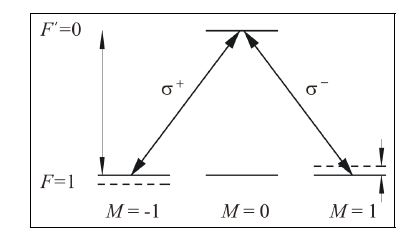
\includegraphics[width=0.75\linewidth]{figures/optical_rotation}
\caption{Illustrative example of F = 1 to $F' = 0$ atomic transition with Zeeman
splitting in the presence of a magnetic field. Image\cite{Budker2002JU2}\label{fig:Zeemansplitting}}
\end{figure}

\subsection{Magneto Optical Rotation}
\bigskip
In the presence of an axial magnetic field, when a linearly polarized light passes through an atomic medium the plane of polarization rotates. This kind of effect is known as the Faraday effect. When Larmor frequencies are smaller than the resonance linewidth, the produced optical rotation is directly proportional to the applied magnetic field which is the main feature of Linear Faraday rotation. We can relate this Faraday effect to the Zeeman shifts in the atomic energy level in the medium. The resonant enhancement of the Faraday rotation has discovered by D. Macaluso and O.M Corbino in 1898 which is known as nonlinear magneto-optical rotation (NMOR) or nonlinear Faraday rotation \cite{budker2013optical}. In the case of linear effect, optical rotation arises due to the absorption of certain contributions of the probe light. On the other hand, the generated disequilibrium in an atom via optical pumping gives rise to nonlinear effect which then alters the birefringent properties of a probe beam. 
As discussed above, the medium is optically pumped into an aligned state, which will
absorb y-polarized light, and not z-polarized light. This is linear dichroism, the differential absorption of orthogonal linear polarizations. On its own this would not affect our probe beam, as it is also polarized in the z-direction. The external B field now modifies the medium. The axis of alignment precesses in a
magnetic field, rotating the axis of dichroism. Finally, the probe beam interacts with the  rotated axis of dichroism, resulting in a rotation of polarization.
The optical rotation can be estimated as
\begin{equation}
\phi \approx \frac{(2g\mu B)/ \hbar\tau)}{(1+((2g\mu B)/(\hbar\tau))^2 )}\frac{l}{l_0}
\end{equation}
where $2g\mu/\hbar$ is correlated to Zeeman splitting, $\tau$ is the doppler width of the
absorption line (of order GHz), and $l_0$ is the absorption length in the medium. 
\begin{figure}
\centering
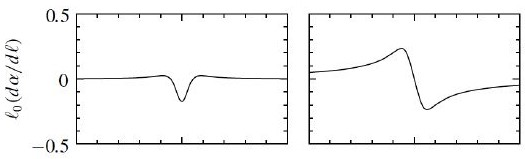
\includegraphics[width=0.85\linewidth]{figures/faraday_rotation}
\caption{Optical rotation in the linear and non-linear case. Image \cite{auzinsh2010optically}\label{fig:optical rotation}}
\end{figure}
The aligned atoms relax after an average time $1/\tau$. In this time, how far around they precess depends on the magnetic field. As the field increases, the precession proceeds further and further, increasing the rotation. As the field becomes high enough to precess the alignment around a full revolution before it decays, the effect starts to average itself out over the ensemble of atoms, and the rotation decreases again. Figure \ref{fig:optical rotation} shows the optical rotation for linear and non-linear Faraday effect. The symmetry of the shape comes from the fact that the precession goes the opposite way for a magnetic field of the opposite sign.
These two effects, the linear effect resulting from circular birefringence, and the nonlinear effect resulting from linear dichroism, represent the two basic mechanisms by which the polarization of the probe beam is rotated. In the zero field case these effects happen simultaneously and continuously, resulting in a steady signal being measured.


\section{Rb magnetometry based on NMOR}

A scalar magnetometer requires coherent precession of the spin ensemble, so a resonant excitation must be applied in order to force some large fraction of the atoms to precess together with a common phase. Otherwise the phase of individual atoms is random, and the total transverse spin of the ensemble averages to zero . The sensitivity of NMOR based atomic magnetometer depends on the lifetime of the polarization state. So in this case, it is important to use ground-state polarization since ground-state polarization has a longer lifetime than the excited states. The working principle of a Rb magnetometer can be described as three step process
\begin{itemize}
\item
Resonant light polarizes Rb atoms via optical pumping. Magnetic
moments of the atoms are oriented with respect to the axis of
alignment
\end{itemize}
\begin{itemize}
\item Aligned magnetic dipole moments experience a torque and precess
  around the axis of the field at the Larmor frequency and medium
  becomes birefringent
\end{itemize}
\begin{itemize}
\item A linearly polarized probe beam propagating parallel to the
pump beam is passed through the alkali vapor, the plane of polarization of the probe beam
rotates by an angle proportional to the spin component along that direction, and we detect
this rotation in order to observe the spin behavior.
optical polarization rotation of a probe beam is used to measure
  magnetic field
\end{itemize}
\begin{figure}[h]
\centering
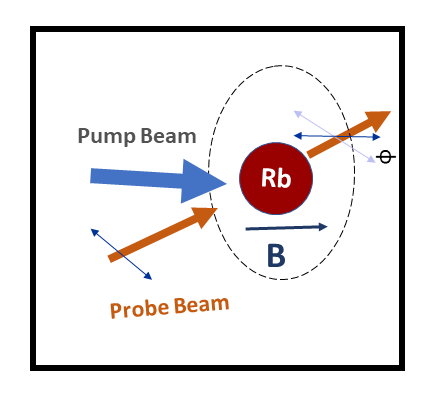
\includegraphics[width=0.55\linewidth]{figures/optical_pumping}
\caption{The schematic diagram of the optical magnetometry technique.
  A linearly polarized pump beam is sent through the vapor cell
  containing natural Rubidium placed in a homogeneous magnetic field
  B.  The polarization rotation of a linearly polarized probe beam is
  used to measure magnetic field}
\end{figure}
